\subsection{Filterspezifikation}
Das Stubfilter ist durch die g-Parameter des Prototypfilters, die Grenzfrequenz (Passband) $f_C$, die Bezugsfrequenz $f_{\frac{\lambda}{4}}$ und die Bezugsimpedanz $Z_0$ vollständig spezifiziert.

\paragraph{g-Parameter}
\begin{mdframed}
\begin{equation*} 
\begin{array}{rclcl} 
g_0 & = & 1 \\ 
g_1 & = & 0.973 \\ 
g_2 & = & 1.372 \\ 
g_3 & = & 1.803 \\ 
g_4 & = & 1.372 \\ 
g_5 & = & 0.973 \\ 
g_6 & = & 1 \\ 
\end{array} 
\end{equation*} 
\end{mdframed}

\paragraph{Bezugsgrössen}
\begin{mdframed}
\begin{equation*} 
\begin{array}{rclcl} 
f_C & = & 0.8 GHz \\ 
f_{\frac{\lambda}{4}} & = & 2GHz \\ 
Z_0 & = & 50 \Omega \\ 
\end{array} 
\end{equation*} 
\end{mdframed}

Die Bezugsgrössen werden erst ab der Richards Frequenztransformation interessant. Anders sieht es aber mit den g-Parametern des Prototypfilters aus. Diese geben Auskunft über Filtertyp, Stopbandrippel und Sperrbandrippel, welche das Stubfilter aufweisen soll. Erst mit Kenntnis dieser Filtereigenschaften kann beurteilt werden, ob das synthetisierte Stubfilter die Filterspezifikationen einhält. Deshalb wird in einem ersten Schritt eine Simulation des Prototypfilter mit den gegebenen g-Parametern durchgeführt, damit Filtertyp, Stopbandrippel und Sperrbandrippel bekannt sind.


Abb. \ref{fig:Topologie_Prototyp.png} illustriert das simulierte Prototyp-Tiefpass-Filter 5. Ordnung mit den Elementwerten  $g_0$ bis $g_6$.

\begin{figure}[h!]
\centering
 	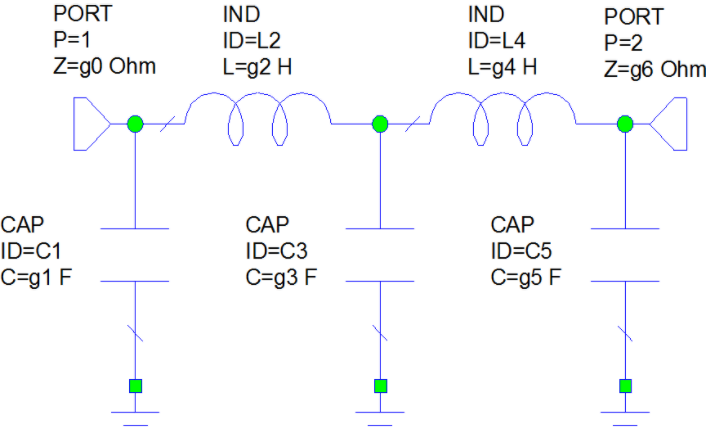
\includegraphics[width=\imagewidth]{images/Topologie_Prototyp.png}
 	\caption{Prototyp-Tiefpass-Filter 5. Ordnung}
 	\label{fig:Topologie_Prototyp.png}
\end{figure}

Die Übersichtsdarstellung der Eingügedämpfung S21 (Abb. \ref{fig:Ovw_Prototyp}) zeigt, dass das Filter keinen Stopbandrippel aufweist. Währenddem die Detailanssicht der Einfügedämpfung S21 in Abb. \ref{fig:Prototyp_Passbandrippel} einen kleinen Equirippel von $-0.04058 dB$ im Passbands sichtbar macht. Dieses Verhalten trifft auf das eines Chebyshev-Filter des Typ I zu, wie aus Abb. \ref{fig:filtertypes.png} unschwer erkennbar ist.

\begin{figure}[h!]
\centering
 	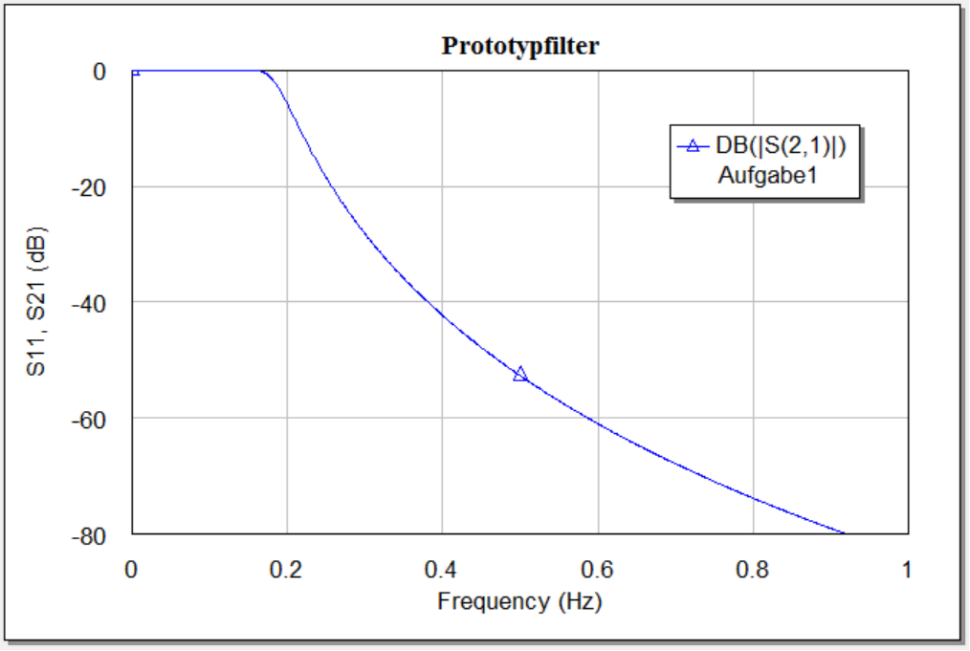
\includegraphics[width=\imagewidth]{images/Ovw_Prototyp.png}
 	\caption{Übersichtsdarstellung S21}
 	\label{fig:Ovw_Prototyp}
\end{figure}

\begin{figure}[h!]
\centering
 	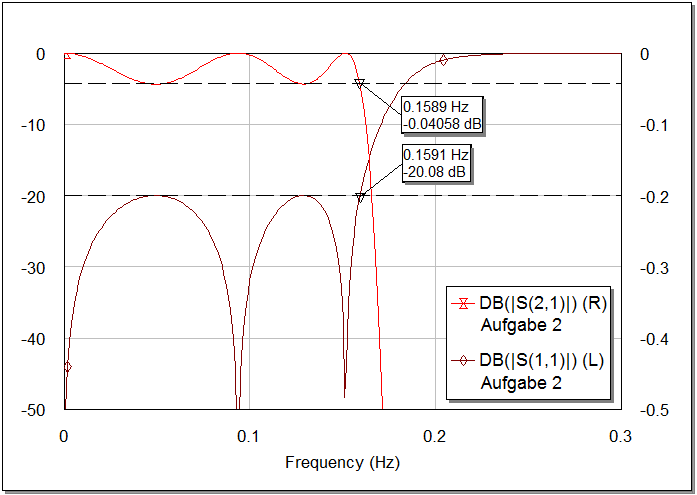
\includegraphics[width=\imagewidth]{images/graph-LC.png}
 	\caption{Detailansicht S21 und S11}
 	\label{fig:graph-LC}
\end{figure}

\begin{figure}[h!]
\centering
 	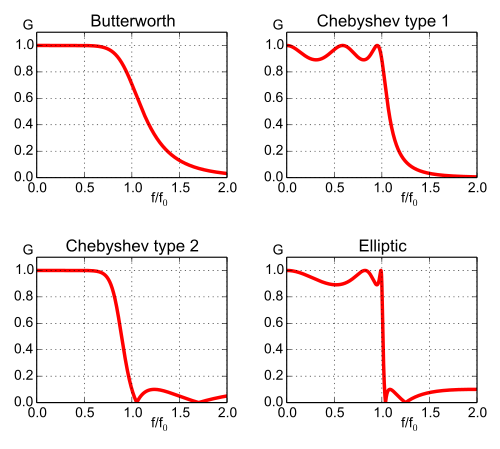
\includegraphics[width=\imagewidth]{images/filtertypes.png}
 	\caption{Filtertypen, \cite{ref:wikipedia:chebyshev}}
 	\label{fig:filtertypes.png}
\end{figure}

Zusammenfassend konnten mithilfe der Simulation also die folgenden Filtereigenschaften des Stubfilters gefunden werden : 

\begin{mdframed}
\begin{equation*} 
\begin{array}{rclcl} 
Filtertyp & = & Chebyshev\ Typ\ I\\
Passbandrippel & = & -0.04058 dB \\ 
Stopbandrippel & = & - 
\end{array} 
\end{equation*} 
\end{mdframed}

\newpage
Ein verlustloses Filter lässt sich nicht nur mit der Einfgedämpfung S21 sondern auch mit der Reflexion S11 beschreiben, weil der folgende Zusammenhang gilt:

\begin{equation}
{|S11|}^2 + {|S21|}^2 = 1
\end{equation}

Somit kann die Reflexion im Passband mithilfe des Equirippels im Passband berechnet werden.

\begin{equation}
|S11(f_C)| = \sqrt{1-{|Equirippel|}^2} = -20 dB
\end{equation}

Um das Resultat zu validieren, wurde die Reflexion S11 des Filters ebenfalls simuliert und in der Detailansicht in  Abb. \ref{fig:graph-LC} dargestellt.







%Beim zu realisierenden Stubfilter handelt es sich um ein Tiefpass-Filter 5. Ordnung, mit einer Grenzfrequenz (Passband) $f_C = 0.8GHz $ und einer Bezugsfrequenz $f_{\frac{\lambda}{4}} = 2GHz$. Die Bezugsfrequenz $f_{\frac{\lambda}{4}}$ definiert die Länge l der gleich langen Leitungsstücke uns ist folglich:

%\begin{equation*}
%l = \frac{\lambda}{4} = \frac{c}{4 \cdot f} = \frac{300\cdot 10^6 \lbrack\frac{m}{s}\rbrack}{4 \cdot 2 \lbrack GHz \rbrack} =37.5 \lbrack mm \rbrack
%\end{equation*}




%\begin{mdframed}
%    \begin{equation*} 
%        \begin{array}{rclcl} 
%            Equirippel & = & -0.04355 dB \\ 
%           \omega_C & = & 1 \\ 
%            f_C & = & 0.1592 Hz \\ 
%        \end{array} 
%    \end{equation*} 
%\end{mdframed}







%Zusammenfassend handelt sich beim zu realisierenden Stubfilter um ein Chebyshev Filter 5. Ordnung des Typ 1 mit folgenden Eigeschaften: 
%\begin{mdframed}
%    \begin{equation*} 
%        \begin{array}{cllll} 
%            f_C & = & 0.8 GHz \\ 
%            f_\frac{\lambda}{4} & = & 2 GHz \\ 
%            l & = & 37.5mm \\
%            Equirippel (Passband) & = & -0.004355 dB \\
%            Reflexion (Passband) & = & -20 dB \\
%        \end{array} 
%    \end{equation*} 
%\end{mdframed}



